\documentclass[]{ctexart}

\usepackage{graphicx} 
\usepackage{xcolor}
\usepackage{listings}
\lstdefinestyle{lfonts}{
	basicstyle   = \footnotesize\ttfamily,
	stringstyle  = \color{purple},
	keywordstyle = \color{blue!60!black}\bfseries,
	commentstyle = \color{olive}\scshape,
}
\lstdefinestyle{lnumbers}{
	numbers     = left,
	numberstyle = \tiny,
	numbersep   = 1em,
	firstnumber = 1,
	stepnumber  = 1,
}
\lstdefinestyle{llayout}{
	breaklines       = true,
	tabsize          = 2,
	columns          = flexible,
}
\lstdefinestyle{lgeometry}{
	xleftmargin      = 20pt,
	xrightmargin     = 0pt,
	frame            = tb,
	framesep         = \fboxsep,
	framexleftmargin = 20pt,
}
\lstdefinestyle{lgeneral}{
	style = lfonts,
	style = lnumbers,
	style = llayout,
	style = lgeometry,
}
\lstdefinestyle{python}{
	language = {Python},
	style    = lgeneral,
}

\title{the Proliferation of Value in Reproduction\newline (再生产中的价值增殖)}
\author{李小狼也是Geek}

\begin{document}

\maketitle

\begin{abstract}

My functions about new surplus value and the rate of profit connect past, now and future of reproduction, describe the permanent proliferation of value in reproduction.

我的关于新剩余价值和利润率的函数，联系了再生产的过去、现在和未来，描述了再生产中价值的不断增殖。

\end{abstract}

\section{the Functions about the Proliferation of Value in Reproduction (再生产中价值增殖的相关函数)}

In general, we have known the normal functions of total capital and the surplus value in \textbf{production}.

一般地，我们已知\textbf{生产}中的总资本和剩余价值的一般函数。

$$capital\_total = c + v$$

$$m = v \times mr$$

In addition, we can get the function of rate of profit in production as follows:

另外，我们可以获得生产中的利润率函数如下：

$$pr = \frac{m}{capital\_total} = \frac{v \times mr}{c + v}$$

But now we add the parameters of \textbf{reproduction} into these functions and therefor enrich themselves. The surplus value had been created in the previous circle of capital is taken partly by capitalist as their personal income, and the rest part of it will be divided into constant and variable capital. 

但现在我们把\textbf{再生产}的一些参数加到这些函数中，从而丰富它们本身。剩余价值在资本的上一次循环中所创造者，一部分被资本家当作他们的个人收入，其余部分又分为不变资本和可变资本。

$$m_p = mg_p - cc_p$$

$$v = v_p + v_{add} = v_p + m_p \times vrr$$

Thus we can get the functions of surplus value and rate of profit in reproduction as follows:

由此可以得到再生产中剩余价值与利润率的函数如下:

$$m = (v_p + (mg_p - cc_p) \times vrr) \times mr$$

$$pr = \frac{m}{c + v} = \frac{(v_p + (mg_p - cc_p) \times vrr) \times mr}{c_p + v_p + mg_p - cc_p}$$

\section{list of parameters (参数列表)}

$capital\_total$: total capital.

$capital\_total$: 总资本。

$c$: \textbf{c}onstant capital in this circle.

$c$: 本次循环中的不变资本。

$v$: \textbf{v}ariable capital in this circle.

$v$: 本次循环中的可变资本。

$m$: surplus value(\textbf{m}) created in this circle.

$m$: 本次循环中创造了的剩余价值。

$mr$: \textbf{r}ate of surplus value(\textbf{m}) in this circle.

$mr$: 本次循环中的剩余价值率。

$pr$: \textbf{r}ate of \textbf{p}rofit in this circle.

$pr$: 本次循环中的利润率。

$c_p$: \textbf{c}onstant capital in \textbf{p}revious circle.

$c_p$: 上次循环中的不变资本。

$v_p$: \textbf{v}ariable capital in \textbf{p}revious circle.

$v_p$: 上次循环中的可变资本。

$mg_p$: \textbf{g}ross surplus value(\textbf{m}) in \textbf{p}revious circle.

$mg_p$: 上次循环中的毛剩余价值。

$m_p$: surplus value(\textbf{m}) in \textbf{p}revious circle.

$m_p$: 上次循环中的剩余价值。

$cc_p$: in\textbf{c}ome of \textbf{c}apitalists in \textbf{p}revious circle.

$cc_p$: 上次循环中的资本家收入。

$v_{add}$: \textbf{v}ariable capital \textbf{a}dded in this circle.

$v_{add}$: 本次循环期初追加的可变资本。

$vrr$: \textbf{r}einvest \textbf{r}ate of surplus value to \textbf{v}ariable capital in this circle.

$vrr$: 本次循环中剩余价值到可变资本的再投资比例。

\section{the Programs of Surplus Value in Reproduction etc. (再生产中的剩余价值之程序云云)}

The function of surplus value in reproduction can be written in Haskell as follow:

再生产中的剩余价值函数可用Haskell写成下面这样：

\textit{m vp mgp ccp vrr mr = (vp + (mgp - ccp) * vrr) * mr},

Or this function can be written in Python to find several relevant economic curves.

或者这一函数可用Python写，来找出若干相关的经济曲线。

\begin{lstlisting}[style = python]
	import matplotlib.pyplot as plt
	import matplotlib as mpl	
\end{lstlisting}

We can find some relations between special parameters. 

我们可以找出特定的参数之间的一些关系。

\begin{figure}[htb]
	\centering
	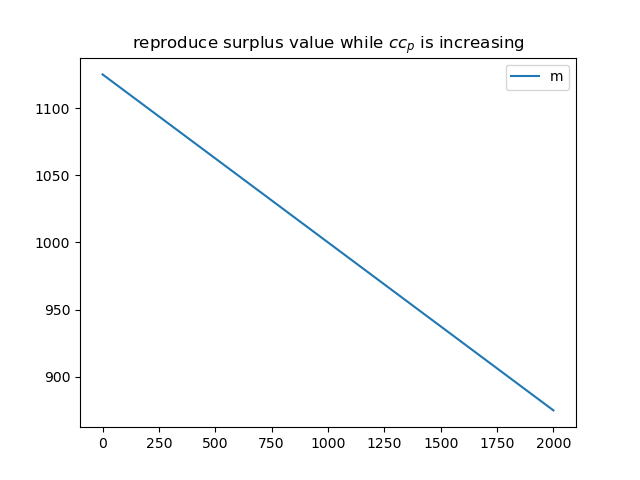
\includegraphics[width=\textwidth]{Figure_1.png}
	\caption{\label{1} reproduce surplus value while $cc_p$ is increasing (当$cc_p$增长时再生产的剩余价值)}
\end{figure}

In the function of surplus value in reproduction, we can find a negative parameter which represents the income of capitalists. That is to say, personal consume of capitalists will hinder the process of proliferation of capital in a certain way. For example, we change the capitalist income($cc_p$) step by step to see the changes of surplus value($m$) influenced by this parameter.

在再生产中的剩余价值的函数中，我们可以找到一个消极的参数，它代表资本家的收入。也就是说，资本家的个人消费会以某种方式阻碍资本的增殖过程。比如，我们一步步地改变资本家的收入（$cc_p$），来观察这个参数所影响的剩余价值（$m$）的改变。

As we can see, the increase of $cc_p$ will decreases $m$.

正如所见，$cc_p$的增加会减少$m$。

\section{Additional or derivative functions (额外的或派生的函数)}

The radio of the rate of surplus value to the rate of profit from the perspective of \textbf{production}:

\textbf{生产}视角下的剩余价值率与利润率之比：

$$\frac{mr}{pr} = (\frac{v}{c + v})^{-1}$$

The radio of the rate of surplus value to the rate of profit from the perspective of \textbf{reproduction}:

\textbf{再生产}视角下的剩余价值率与利润率之比：

$$\frac{mr}{pr} = (\frac{v_p + (mg_p - cc_p) \times vrr}{c_p + v_p + mg_p - cc_p})^{-1}$$

Index $-1$ can not only complicates but also simplifies these functions and show the relations between $mr$ and $pr$ more clearly, so it is proper to use this index.

指数$-1$不仅可以复杂化也可以简化这些函数，并且更清晰地展现$mr$与$pr$之间的关系，所以用这个指数是合适的。

\section{Conclusion (结论)}

These function can only show some aspects of production and get rid of many important parameters and relations. So we should recognize these functions as special moments of logic.

这些函数只能反映生产的某些方面，并排除了许多重要的参数和关系。所以我们应该将这些函数认作特殊的逻辑环节。

For instance, it is critical to realize that the rate of variable capital will reduce continually in the total process of reproduction, etc.

例如，在整个再生产过程中，可变资本的比率会持续下降，等等。认识到这一点，是紧要的。


And these functions are kind of recursion, because the surplus value created now can be set as the original parameter in these functions themselves and then joins the next reproduction.

并且这些函数是一种递归，因为现在创造的剩余价值可以被设置为这些函数本身中的初始参数，并这样加入下次的再生产。

It seems that the reproduction of capitalism is infinite, but this point of view is innocent. The system of capitalism has its inner limits and will be destroyed by its own development.

看起来，资本主义的再生产是无限的，但这种观点是天真的。资本主义体系有其内在的局限性，并将被自身的发展所毁灭。

%切切实实地发展了马克思的再生产理论，着重讨论了其中剩余价值等的一般运动。

\end{document}
